\documentclass{beamer}

\DeclareMathOperator{\Lapl}{\mathcal{L}}
\DeclareMathOperator{\Real}{\mathbb{R}}

\usepackage{algorithm}
\usepackage{algorithmic}
\renewcommand{\algorithmicrequire}{\bf{Input:}}
\renewcommand{\algorithmicensure}{\bf{Output:}}

\usepackage{pgfplots}
\usepgfplotslibrary{groupplots}

\setbeamercolor{footline}{fg=blue}
\setbeamerfont{footline}{series=\bfseries}
\addtobeamertemplate{navigation symbols}{}{
    \usebeamerfont{footline}
    \usebeamercolor[fg]{footline}
    \hspace{2em}
    \insertframenumber/\inserttotalframenumber
}

\title{Image Processing using Graph Laplacian Operator}
\author{David Wobrock}
\institute{ALPINES Team - INRIA Paris \\ Laboratoire Jacques-Louis Lions - Sorbonne Universit\'e \\ KTH, Stockholm \\ INSA Lyon}
\date{\today}

\begin{document}

\frame{\titlepage}

\begin{frame}
 \frametitle{Table of Contents}
 \tableofcontents
\end{frame}

\section[Section]{Introduction}

\begin{frame}
 \frametitle{Background}
 \begin{itemize}
  \item Millions of pictures shared daily
  \item Image processing using spectral methods on smartphones (denoising, sharpening, ...)
  \item Involves eigenvalue problems, linear algebra and solving dense linear systems
  \item Opportunity for high-performance computing and parallelism
 \end{itemize}
\end{frame}

\begin{frame}
 \frametitle{Objective}
 \begin{itemize}
  \item Not necessarily improving image processing
  \item Analyse the behaviour of solving large dense systems
 \end{itemize}
 \begin{itemize}
  \item Large: \(N^2\), \(N\) the number of pixels in the input image
  \item Dense: affinity and Laplacian matrices are dense because global filter
 \end{itemize}
\end{frame}

\section[Section]{Image processing using Laplacian operator}

\begin{frame}
 \frametitle{Image processing - Global filter algorithm}
 \begin{itemize}
  \item \(z\) output image, \(y\) input image, \(W\) data-dependent global filter of size \(N^2\)
  \item \(z_i = \sum^{N}_{j=1} W_{ij}y_j\)
  \item A vector of weights for each pixel
  \item Global filter: \(z = Wy\)
 \end{itemize}
\end{frame}

\begin{frame}
 \frametitle{Image processing - Image as graph}
 \begin{itemize}
  \item Think of the image as a graph
  \item Each pixel is a node
  \item The graph is complete and the edges are weighted
  \item The weight represents the similarity between two pixels/nodes
  \item Similarity can be measured by weighting together spatial and color closeness of pixels
  \item Bilateral kernel: \(exp(-\frac{||x_i - x_j||^2}{h_x^2}) \cdot exp(-\frac{||z_i - z_j||^2}{h_z^2})\)
 \end{itemize}
\end{frame}

\begin{frame}
 \frametitle{Image processing - Filter and Laplacian}
 \begin{itemize}
  \item \(K\) affinity matrix, \(\Lapl\) Laplacian matrix, \(W\) filter matrix and \(f\) a function
  \item Filter defined as \(W = I - f(\Lapl)\)
  \item Let \(d_i = \sum_j K_{ij}\), \(D = diag\{d_i\}\) and \(\bar{d} = \frac{1}{N} \sum_i d_i\)
 \end{itemize}
 \begin{table}
  \centering
  \begin{tabular}{|c|c|c|c|c|}
   \hline
   Laplacian & Formula of \(\Lapl\) & Symmetric & Spectral Range \\
   \hline
   Un-normalised & \(D - K\) & Yes & [0, n] \\
   \hline
   Normalised & \(I - D^{-1/2}KD^{-1/2}\) & Yes & [0, 2] \\
   \hline
   Random walk & \(I - D^{-1}K\) & No & [0, 1] \\
   \hline
   ``Sinkhorn'' & \(I - C^{-1/2}KC^{-1/2}\) & Yes & [0, 1] \\
   \hline
   Re-normalised & \(\alpha(D - K)\), \(\alpha \approx \bar{d}^-1\) & Yes & [0, n] \\
   \hline
  \end{tabular}
  \caption{Overview of different graph Laplacian operator definitions.}
 \end{table}
\end{frame}

\begin{frame}
 \frametitle{Image processing - Sampling and Nystr\"om extension}
 \begin{itemize}
  \item Sample \(p\) pixels of the image (\(\le 1\%\) of pixels)
  \item With \(K_A \in \Real^{p \times p}\),\(K_B \in \Real^{p \times N-p}\) and \(K_C \in \Real^{N-p \times N-p}\) \(K = \begin{bmatrix}K_A & K_B \\ K_B^T & K_C\end{bmatrix}\)
  \item Approximate \(K\) by \(\tilde{K} = \tilde{\Phi} \tilde{\Pi} \tilde{\Phi^T}\)
  \item With submatrix \(K_A = \Phi_A \Pi_A \Phi_A^T\), \\
   \(\tilde{\Pi} = \Pi_A\) \\
   \(\tilde{\Phi} = \begin{bmatrix}\Phi_A \\ K_B^T \Phi_A \Pi_A^{-1} \end{bmatrix}\)
  \item Finally, \(\tilde{K} = \begin{bmatrix} K_A & K_B \\ K_B^T & K_B^T K_A^{-1} K_B \end{bmatrix}\)
 \end{itemize}
\end{frame}

\begin{frame}
 \frametitle{Image processing - Eigenvalues}
 \begin{itemize}
  \item For the filter, only the largest eigenvalues are needed because the smallest tends to 0
  \item There is an equivalence between largest eigenvalues of \(W\) and the smallest ones of \(\Lapl\)
  \item The smallest eigenvalues can be computed with the inverse power method, which requires solving systems of linear equations
  \item But the Nystr\"om extension only works for leading eigenvalues.
 \end{itemize}
\end{frame}

\begin{frame}
 \frametitle{Image processing - Algorithm recap}
  \begin{algorithm}[H]
   \caption{Image processing using approximated graph Laplacian operator}
   \begin{algorithmic}
    \REQUIRE \(y\) an image of size \(N\), \(f\) the function applied to \(\Lapl\)
    \ENSURE \(\tilde{z}\) the output image by the approximated filter
    \STATE \COMMENT{Sampling}
    \STATE Sample \(p\) pixels, \(p \ll N\)
    \STATE \COMMENT{Kernel matrix approximation}
    \STATE Compute \(K_A\) (size \(p \times p\)) and \(K_B\) (size \(p \times (N-p)\))
    \STATE Compute the Laplacian submatrices \(\Lapl_A\) and \(\Lapl_B\)
    \STATE \COMMENT{Eigendecomposition}
    \STATE Compute the \(m\) smallest eigenvalues \(\Pi_A\) and the associated eigenvectors \(\Phi_A\) of \(\Lapl_A\)
    \STATE \COMMENT{Nystr\"om extension and compute the filter}
    \STATE See methods of solution proposed by Fowlkes, 2004
    \STATE \(\tilde{z} \leftarrow \tilde{W} y\)
   \end{algorithmic}
\end{algorithm}
\end{frame}


\section[Section]{Parallel implementation}

\begin{frame}
 \frametitle{Parallel implementation details}
 \begin{itemize}
  \item C language
  \item PETSc (Toolkit for scientific computing in parallel)
  \item SLEPc, Elemental
 \end{itemize}
\end{frame}

\begin{frame}
 \frametitle{Full matrix computation result}
 \begin{figure}[H]
  \centering
  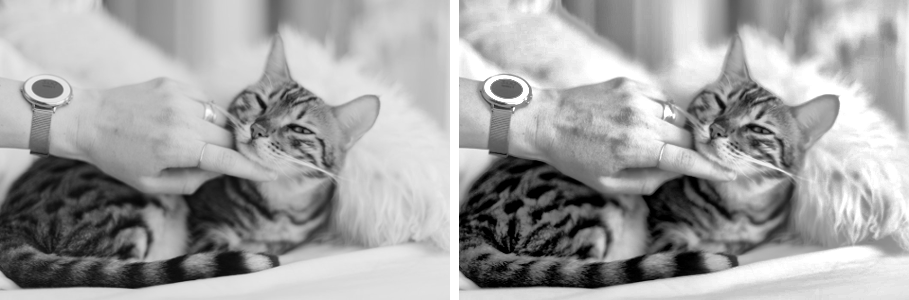
\includegraphics[width=0.95\textwidth]{../master_thesis/img/cat.png}
  \caption{Left: input image. Right: sharpened image.}
 \end{figure}
\end{frame}

\begin{frame}
 \frametitle{Runtime of full matrix computation}
 \begin{figure}[H]
  \centering
  \begin{tikzpicture}
 \begin{axis}[
  xlabel=Number of processors,
  xtick={16, 32, 64, 96, 128, 192},
  xmode=log,
  ymode=log,
  log ticks with fixed point,
  ylabel=Total runtime (seconds)]
   \addplot[color=blue, mark=x] coordinates {
    %(1, )
    %(2, )
    %(4, )
    %(8, )
    (16, 646.344379)
    (32, 338.1412974)
    (64, 173.1325498)
    (96, 121.8080638)
    (128, 91.1042946)
    (160, 76.0524958)
    (192, 66.9623342)
   };
 \end{axis}
\end{tikzpicture}

  \caption{Total runtime of the algorithm with entire matrix computation (log scale).}
 \end{figure}
\end{frame}

\begin{frame}
 \frametitle{Inverse subspace iteration}
 \begin{algorithm}[H]
  \caption{Inverse subspace iteration}
  \begin{algorithmic}
   \REQUIRE \(A\) the matrix of size \(p \times p\), \(m\) the number of required eigenvalues, \(\varepsilon\) a tolerance
   \ENSURE \(X_k\) the desired invariant subspace
   \STATE Initialise \(m\) random orthonormal vectors \(X_0\) of size \(p\)
   \STATE \(R_0 \gets (I - X_0 X_0^T) A X_0\)
   \STATE For k=0, 1, 2, \dots
   \WHILE{\(\|R_k\| > \varepsilon\)}
    \FOR{i=1 \TO m}
     \STATE Solve \(A X_{k+1}^{(i)} = X_k^{(i)}\)
    \ENDFOR
    \STATE \(X_{k+1} \gets \) Orthonormalise(\(X_{k+1}\))
    \STATE \(R_{k+1} \gets (I - X_{k+1} X_{k+1}^T) A X_{k+1}\)
   \ENDWHILE
  \end{algorithmic}
 \end{algorithm}
\end{frame}

\begin{frame}
 \frametitle{Approximation runtime of approximated computation}
 \begin{figure}[H]
  \centering
  \begin{tikzpicture}
 \begin{groupplot}[
  group style={
   group size=2 by 1,
   xlabels at=edge bottom,
   ylabels at=edge left,
   horizontal sep=1.5cm,
   },
  height=6cm,
  width=0.5\textwidth,
  xlabel=Number of processors,
  xtick={2, 4, 8, 16, 32, 64, 128},
  xmode=log,
  ymode=log,
  log ticks with fixed point,
  ylabel=Runtime (seconds)
  ]
  \nextgroupplot[title={50 eigenvalues.}]
   \addplot[color=blue, mark=x] coordinates {
    (2, 772.1529408)
    (4, 381.4875584)
    (8, 196.6197338)
    (16, 104.6891928)
    (32, 59.8903464)
    (64, 35.9956886)
    (96, 29.214667)
    (128, 25.4793632)
    (160, 24.0418716)
    (192, 23.1824056)
   };

  \nextgroupplot[title={500 eigenvalues.}]
   \addplot[color=blue, mark=x] coordinates {
    (2, 7149.885403)
    (4, 5149.912356)
    (8, 4373.481026)
    (16, 3903.60577)
    (32, 3803.859549)
    (64, 3712.591258)
    (96, 3824.621957)
    (128, 3939.533307)
    (160, 3986.572888)
    (192, 4383.063958)
   };
 \end{groupplot}
\end{tikzpicture}

  \caption{Runtime of the inverse subspace iteration part of the algorithm (log scale).}
 \end{figure}
\end{frame}

\begin{frame}
 \frametitle{Runtime in the inverse subspace iteration algorithm}
 \begin{figure}[H]
  \centering
  \scalebox{0.8}{\begin{tikzpicture}
 \begin{groupplot}[
  group style={
   group size=2 by 1,
   xlabels at=edge bottom,
   ylabels at=edge left,
   },
  ybar stacked,
  ymin=0,
  ymax=100,
  height=7cm,
  width=0.5\textwidth,
  xlabel=Number of processors,
  ylabel={Percentage (\%)},
  symbolic x coords={2, 4, 8, 16, 32, 64, 96, 128, 160, 192},
  legend style={
   at={(0, -0.25)},
   anchor=north}
  ]
  \nextgroupplot[title={50 eigenvalues.}]
  \addplot[ybar, fill=blue] plot coordinates {
   (2, 8.14)
   (4, 6.16)
   (8, 5.98)
   (16, 9.09)
   (32, 13.50)
   (64, 18.56)
   (96, 22.42)
   (128, 25.35)
   (160, 27.53)
   (192, 29.06)};
  \addplot[ybar, fill=red] plot coordinates {
   (2, 0.46)
   (4, 0.96)
   (8, 2.01)
   (16, 3.90)
   (32, 7.31)
   (64, 13.29)
   (96, 17.61)
   (128, 20.94)
   (160, 23.90)
   (192, 26.27)};
  \addplot[ybar, fill=yellow] plot coordinates {
   (2, 85.67)
   (4, 86.96)
   (8, 86.16)
   (16, 81.40)
   (32, 73.91)
   (64, 63.23)
   (96, 55.21)
   (128, 49.07)
   (160, 43.95)
   (192, 40.00)};
  \addplot[ybar, fill=green] plot coordinates {
   (2, 5.74)
   (4, 5.92)
   (8, 5.84)
   (16, 5.61)
   (32, 5.28)
   (64, 4.91)
   (96, 4.76)
   (128, 4.64)
   (160, 4.62)
   (192, 4.68)};

  \nextgroupplot[title={500 eigenvalues.}]
  \addplot[ybar, fill=blue] plot coordinates {
   (2, 23.76)
   (4, 15.29)
   (8, 11.43)
   (16, 12.30)
   (32, 11.68)
   (64, 9.84)
   (96, 9.47)
   (128, 9.75)
   (160, 9.57)
   (192, 9.39)};
  \addplot[ybar, fill=red] plot coordinates {
   (2, 46.02)
   (4, 63.07)
   (8, 75.14)
   (16, 79.65)
   (32, 83.37)
   (64, 86.81)
   (96, 87.72)
   (128, 87.77)
   (160, 88.07)
   (192, 88.50)};
  \addplot[ybar, fill=yellow] plot coordinates {
   (2, 28.78)
   (4, 20.15)
   (8, 11.97)
   (16, 6.60)
   (32, 3.49)
   (64, 1.84)
   (96, 1.29)
   (128, 0.98)
   (160, 0.80)
   (192, 0.64)};
  \addplot[ybar, fill=green] plot coordinates {
   (2, 1.44)
   (4, 1.48)
   (8, 1.46)
   (16, 1.46)
   (32, 1.46)
   (64, 1.51)
   (96, 1.53)
   (128, 1.50)
   (160, 1.56)
   (192, 1.47)};
  \legend{
   Solving the system of linear equations,
   Gram-Schmidt orthogonalisation,
   Residual norm computation,
   Rest overhead}
 \end{groupplot}
\end{tikzpicture}
}
  \caption{Proportion of each step in the inverse subspace iteration.}
 \end{figure}
\end{frame}

\begin{frame}
 \frametitle{Skipping the Gram-Schmidt procedure}
  \begin{figure}[H]
  \centering
  \begin{tikzpicture}
 \begin{groupplot}[
  group style={
   group size=2 by 1,
   xlabels at=edge bottom,
   ylabels at=edge left,
   horizontal sep=1.5cm,
   },
  height=6cm,
  width=0.5\textwidth,
  xlabel=Number of processors,
  xtick={2, 4, 8, 16, 32, 64, 128},
  xmode=log,
  ymode=log,
  log ticks with fixed point,
  ylabel=Runtime (seconds)
  ]
  \nextgroupplot[title={50 eigenvalues.}]
   \addplot[color=blue, mark=x] coordinates {
    (2, 819.1718588)
    (4, 404.5779052)
    (8, 207.887785)
    (16, 109.2656354)
    (32, 61.5224218)
    (64, 35.5858806)
    (96, 28.0760846)
    (128, 24.3417164)
    (160, 22.365463)
    (192, 21.1874868)
   };

  \nextgroupplot[title={500 eigenvalues.}]
   \addplot[color=blue, mark=x] coordinates {
    (2, 5613.950337)
    (4, 3614.57139)
    (8, 2804.417351)
    (16, 2346.925115)
    (32, 2223.999989)
    (64, 2104.544023)
    (96, 2148.624336)
    (128, 2264.674778)
    (160, 2226.515463)
    (192, 2494.121987)
   };
 \end{groupplot}
\end{tikzpicture}

  \caption{Runtime of the inverse subspace iteration with skipping the Gram-Schmidt procedure every other iteration (log scale).}
 \end{figure}
\end{frame}

\begin{frame}
 \frametitle{Skipping Gram-Schmidt more often}
 \begin{figure}[H]
  \centering
  \scalebox{0.8}{\begin{tikzpicture}
 \begin{groupplot}[
  group style={
   group size=2 by 1,
   xlabels at=edge bottom,
   ylabels at=edge left,
   horizontal sep=2.2cm,
   },
  height=6cm,
  width=0.5\textwidth,
  xlabel={Orthogonalisation every \(x\) iterations},
  xtick={1, 2, 3, 4, 5},
  %xmode=log,
  %ymode=log,
  %log ticks with fixed point,
  ylabel=Runtime (seconds),
  legend style={
   at={(1, -0.3)},
   anchor=north
  },
  ]
  \nextgroupplot[title={2 processors, 500 eigenvalues.}]
   \addplot[color=blue, mark=x] coordinates {
    (1, 7149.885403)
    (2, 5613.950337)
    (3, 0)
    (4, 0)
    (5, 0)
   };
   \addlegendentry{Runtime}
   \addplot[color=black, domain=1:5, dashed] expression {
    7149.885403/x};
   \addlegendentry{Linear speedup}

  \nextgroupplot[title={64 processors, 500 eigenvalues.}]
   \addplot[color=blue, mark=x] coordinates {
    (1, 3712.591258)
    (2, 2104.544023)
    (3, 0)
    (4, 0)
    (5, 0)
   };
   \addplot[color=black, domain=1:5, dashed] expression {
    3712.591258/x};
 \end{groupplot}
\end{tikzpicture}

}
  \caption{Runtime of the inverse subspace iteration depending on the amount of Gram-Schmidt procedures.}
  \end{figure}
\end{frame}

\begin{frame}
 \frametitle{Linear solver performances}
 \begin{figure}[H]
  \centering
  \scalebox{0.95}{\begin{tikzpicture}
 \begin{axis}[
  height=6cm,
  width=\textwidth,
  xlabel=Number of processors,
  xtick={2, 4, 8, 16, 32, 64, 128, 192},
  xmode=log,
  ymode=log,
  log ticks with fixed point,
  ylabel=Runtime (seconds),
  legend style={
   at={(0.5, -0.3)},
   anchor=north
  }]
   \addplot[color=blue, mark=x] coordinates {
    (2, 5.019035956)
    (4, 2.489311578)
    (8, 1.295918689)
    (16, 0.8153684889)
    (32, 0.4725504889)
    (64, 0.3680468222)
    (96, 0.4586239333)
    (128, 0.2866520667)
    (160, 0.3435106444)
    (192, 0.4434605778)
   };
   \addlegendentry{GMRES without preconditioner}
   \addplot[color=red, mark=o] coordinates {
    (2, 4.171304311)
    (4, 1.562855289)
    (8, 0.78404696)
    (16, 0.6342229867)
    (32, 0.5220878222)
    (64, 0.4143123111)
    (96, 0.4201508889)
    (128, 0.4034540222)
    (160, 0.4217084444)
    (192, 0.4490838667)
   };
   \addlegendentry{GMRES + RAS with GMRES on subdomains}
   \addplot[color=yellow, mark=triangle*] coordinates {
    (2, 1.583247378)
    (4, 0.7071820222)
    (8, 0.3530209556)
    (16, 0.2730702667)
    (32, 0.193635)
    (64, 0.1572552667)
    (96, 0.1740185111)
    (128, 0.1541527111)
    (160, 0.1782941778)
    (192, 0.1908772667)
   };
   \addlegendentry{GMRES + RAS with LU factorisation on subdomains}
   \addplot[color=black, domain=2:192, dashed] expression {
    4.171304311*2/x};
   \addlegendentry{Linear speedup}
   \addplot[color=black, domain=2:192, dashed] expression {
    1.583247378*2/x};
 \end{axis}
\end{tikzpicture}
}
  \caption{Runtime of the linear solver for 50 eigenvalues for a \(4000 \times 4000\) matrix (log scale).}
 \end{figure}
\end{frame}

\begin{frame}
 \frametitle{Linear solver performances - big image}
 \begin{figure}[H]
  \centering
  \scalebox{0.95}{\begin{tikzpicture}
 \begin{axis}[
  height=6cm,
  width=\textwidth,
  xlabel=Number of processors,
  xtick={2, 4, 8, 16, 32, 64, 128, 192},
  xmode=log,
  ymode=log,
  log ticks with fixed point,
  ylabel=Runtime (seconds),
  legend style={
   at={(0.5, -0.3)},
   anchor=north
  }]
   \addplot[color=blue, mark=x] coordinates {
    (2, 0)
    (4, 0)
    (8, 0)
    (16, 0)
    (32, 0)
    (64, 0)
    (96, 0)
    (128, 0)
    (160, 0)
    (192, 0)
   };
   \addlegendentry{GMRES without preconditioner}
   \addplot[color=red, mark=o] coordinates {
    (2, 0)
    (4, 0)
    (8, 0)
    (16, 0)
    (32, 0)
    (64, 0)
    (96, 0)
    (128, 0)
    (160, 0)
    (192, 0)
   };
   \addlegendentry{GMRES + RAS with GMRES on subdomains}
   \addplot[color=yellow, mark=triangle*] coordinates {
    (2, 0)
    (4, 0)
    (8, 0)
    (16, 0)
    (32, 0)
    (64, 0)
    (96, 0)
    (128, 0)
    (160, 0)
    (192, 0)
   };
   \addlegendentry{GMRES + RAS with LU factorisation on subdomains}
   \addplot[color=black, domain=2:192, dashed] expression {
    1*2/x};
   \addlegendentry{Linear speedup}
 \end{axis}
\end{tikzpicture}
}
  \caption{Runtime of the linear solver for 50 eigenvalues for a \(14400 \times 14400\) matrix (log scale).}
 \end{figure}
\end{frame}

\section[Section]{Conclusion}

\begin{frame}
 \frametitle{Discussions \& perspectives}
 \begin{itemize}
  \item Linear solver with domain decomposition methods as preconditioner
  \item Skipping Gram-Schmidt
 \end{itemize}
 \begin{itemize}
  \item Finished image processing algorithm
  \item State-of-the-art performances with a similar method
  \item Explore more solvers, domain decomposition methods and other preconditioner
 \end{itemize}
\end{frame}

\end{document}
